\newcommand{\spywareTagResultsAucTable}{
    \begin{table}[h!]
        \centering
        \begin{tabular}{|p{2,8cm}||P{2,2cm} P{2,2cm} P{2,2cm} P{2,2cm}|}
            \hline
            Spyware Tag & ALOHA\newline (M/B only) & ALOHA & Joint\newline Embedding & Proposed\newline Model \\
            \hline
            AUC-ROC & - & 0.960$\pm$0.002 & \textBF{0.970$\pm$0.002} & 0.959$\pm$0.008 \\
            \hline
        \end{tabular}
        \caption[Spyware Tag prediction task AUC-ROC results]{AUC-ROC (Area Under Curve) of the different models for the \textbf{Spyware Tag} prediction task. Results were aggregated over \textBF{3} training runs with different weight initializations and minibatch orderings. Best results are shown in \textbf{bold}.} \label{tab:spywareTag_auc}
    \end{table}
}

\newcommand{\spywareTagResultsAtFprTable}{
    \begin{center}[h!]
        \begin{longtable}[c]{|P{3,2cm}||P{1,8cm} P{1,8cm} P{1,8cm} P{1,8cm} P{1,8cm}|}
            \hline
            Spyware Tag & \multicolumn{5}{c|}{{FPR}} \\
            & $10^{-5}$ & $10^{-4}$ & $10^{-3}$ & $10^{-2}$ & $10^{-1}$ \\
            \hline
            \endfirsthead

            \caption*{\raggedright ...continued from previous page} \\
            \hline
            Spyware Tag & \multicolumn{5}{c|}{\textbf{FPR}} \\
            & $10^{-5}$ & $10^{-4}$ & $10^{-3}$ & $10^{-2}$ & $10^{-1}$ \\
            \hline
            \endhead

            \caption*{\raggedleft ...continued on next page} \\
            \endfoot

            \caption[Spyware Tag prediction task results]{Mean and standard deviation results (TPR, Accuracy, Recall, Precision and F1-Score) of the different models for the \textbf{Spyware Tag} prediction task at different \textbf{FPR}s (\textit{False Positive Rates}). Results were aggregated over \textBF{3} training runs with different weight initializations and minibatch orderings. Best results are shown in \textbf{bold}. Under \textbf{TPR} results are also presented the percentage reduction in mean detection error and in ROC curve standard deviation introduced by the \textit{Proposed Model} with respect to both \textit{ALOHA} model and \textit{Joint Embedding}.} \label{tab:spywareTag_results_at_fpr} \\
            \endlastfoot

            \multicolumn{6}{|c|}{\textbf{TPR}} \\
            \hline
            ALOHA (M/B only) & - & - & - & - & - \\
            ALOHA & 0.086$\pm$0.058 & 0.097$\pm$0.049 & 0.098$\pm$0.049 & 0.604$\pm$0.007 & 0.884$\pm$0.014 \\
            Joint Embedding & \textBF{0.142$\pm$0.065} & \textBF{0.282$\pm$0.087} & \textBF{0.337$\pm$0.130} & 0.662$\pm$0.017 & \textBF{0.910$\pm$0.015} \\
            Proposed Model & 0.101$\pm$0.094 & 0.190$\pm$0.098 & 0.192$\pm$0.099 & \textBF{0.670$\pm$0.019} & 0.887$\pm$0.013 \\
            \hline
            Error Reduction wrt\newline ALOHA (M/B only) & - & - & - & - & - \\
            Error Reduction wrt\newline ALOHA & 1.6\% & 10.3\% & 10.4\% & 16.7\% & 2.6\% \\
            Error Reduction wrt\newline Joint Embedding & -4.8\% & -12.8\% & -21.9\% & 2.4\% & -25.6\% \\
            \hline
            Std Reduction wrt\newline ALOHA (M/B only) & - & - & - & - & - \\
            Std Reduction wrt\newline ALOHA & -62.1\% & -100.0\% & -102.0\% & -171.4\% & 7.1\% \\
            Std Reduction wrt\newline Joint Embedding & -44.6\% & -12.6\% & 23.8\% & -11.8\% & 13.3\% \\
            \hline
            \multicolumn{6}{|c|}{\textbf{Accuracy}} \\
            \hline
            ALOHA (M/B only) & - & - & - & - & - \\
            ALOHA & 0.902$\pm$0.006 & 0.903$\pm$0.005 & 0.903$\pm$0.005 & 0.949$\pm$0.001 & 0.898$\pm$0.001 \\
            Joint Embedding & \textBF{0.908$\pm$0.007} & \textBF{0.923$\pm$0.009} & \textBF{0.928$\pm$0.014} & 0.955$\pm$0.002 & \textBF{0.901$\pm$0.002} \\
            Proposed Model & 0.904$\pm$0.010 & 0.913$\pm$0.011 & 0.913$\pm$0.011 & \textBF{0.956$\pm$0.002} & 0.899$\pm$0.001 \\
            \hline
            \multicolumn{6}{|c|}{\textbf{Recall}} \\
            \hline
            ALOHA (M/B only) & - & - & - & - & - \\
            ALOHA & 0.086$\pm$0.058 & 0.097$\pm$0.049 & 0.098$\pm$0.049 & 0.604$\pm$0.007 & 0.884$\pm$0.014 \\
            Joint Embedding & \textBF{0.142$\pm$0.065} & \textBF{0.282$\pm$0.087} & \textBF{0.337$\pm$0.130} & 0.662$\pm$0.017 & \textBF{0.910$\pm$0.015} \\
            Proposed Model & 0.101$\pm$0.094 & 0.190$\pm$0.099 & 0.192$\pm$0.099 & \textBF{0.670$\pm$0.019} & 0.887$\pm$0.013 \\
            \hline
            \multicolumn{6}{|c|}{\textbf{Precision}} \\
            \hline
            ALOHA (M/B only) & - & - & - & - & - \\
            ALOHA & 0.999$\pm$0.001 & 0.992$\pm$0.004 & 0.908$\pm$0.033 & 0.878$\pm$0.001 & 0.514$\pm$0.004 \\
            Joint Embedding & \textBF{0.999$\pm$0.000} & \textBF{0.997$\pm$0.001} & \textBF{0.971$\pm$0.014} & 0.888$\pm$0.003 & \textBF{0.521$\pm$0.004} \\
            Proposed Model & 0.998$\pm$0.002 & 0.994$\pm$0.003 & 0.940$\pm$0.039 & \textBF{0.889$\pm$0.003} & 0.515$\pm$0.004 \\
            \hline
            \multicolumn{6}{|c|}{\textbf{F1 Score}} \\
            \hline
            ALOHA (M/B only) & - & - & - & - & - \\
            ALOHA & 0.152$\pm$0.097 & 0.173$\pm$0.079 & 0.174$\pm$0.079 & 0.716$\pm$0.005 & 0.650$\pm$0.007 \\
            Joint Embedding & \textBF{0.243$\pm$0.098} & \textBF{0.432$\pm$0.111} & \textBF{0.486$\pm$0.153} & 0.759$\pm$0.012 & \textBF{0.663$\pm$0.007} \\
            Proposed Model & 0.170$\pm$0.150 & 0.307$\pm$0.144 & 0.308$\pm$0.142 & \textBF{0.764$\pm$0.013} & 0.652$\pm$0.007 \\
            \hline
        \end{longtable}
    \end{center}
}

\newcommand{\spywareTagResultsSummaryTable}{
    \begin{table}[h!]
        \centering
        \begin{tabular}{|P{3,2cm}||P{1,8cm} P{1,8cm} P{1,8cm} P{1,8cm} P{1,8cm}|}
            \hline
            \multicolumn{6}{|c|}{Spyware Tag (at FPR $=1\%$)} \\
            \hline
            Model & TPR & Accuracy & Precision & Recall & F1 score \\
            \hline
            ALOHA (M/B only) & - & - & - & - & - \\
            ALOHA & 0.604$\pm$0.007 & 0.949$\pm$0.001 & 0.878$\pm$0.001 & 0.604$\pm$0.007 & 0.716$\pm$0.005 \\
            Joint Embedding & 0.662$\pm$0.017 & 0.955$\pm$0.002 & 0.888$\pm$0.003 & 0.662$\pm$0.017 & 0.759$\pm$0.012 \\
            Proposed Model & \textBF{0.670$\pm$0.019} & \textBF{0.956$\pm$0.002} & \textBF{0.889$\pm$0.003} & \textBF{0.670$\pm$0.019} & \textBF{0.764$\pm$0.013} \\
            \hline
        \end{tabular}
        \caption[Summary of Spyware Tag prediction task results]{Summary of the mean and standard deviation results of the different models for the \textbf{Spyware Tag} prediction task at \textbf{FPR} $=1\%$. Results were aggregated over \textBF{3} training runs with different weight initializations and minibatch orderings. Best results are shown in \textbf{bold}.} \label{tab:spywareTag_result_summary}
    \end{table}
}

\newcommand{\spywareTagRocAlohaMB}{
    \begin{figure}[h!]
        \vspace*{-0.5cm}
        \centering
        \includegraphics[width=0.6\textwidth]{./results/spyware_tag_roc_alohaMB.png}
        \vspace*{-0.2cm}
        \caption[Spyware Tag prediction task ALOHA (M/B only) ROC curve]{ROC curve and AUC statistics of \textBF{ALOHA (M/B only)} model for the \textbf{Spyware Tag}. The line represents the \textit{mean} TPR at a given FPR, while the shaded region represents the \textit{standard deviation}. Statistics were computed over \textBF{3} training runs, each with random parameter initialization.}
        \label{fig:spywareTagRocAlohaMB}
    \end{figure}
}

\newcommand{\spywareTagRocAloha}{
    \begin{figure}[h!]
        \vspace*{-0.5cm}
        \centering
        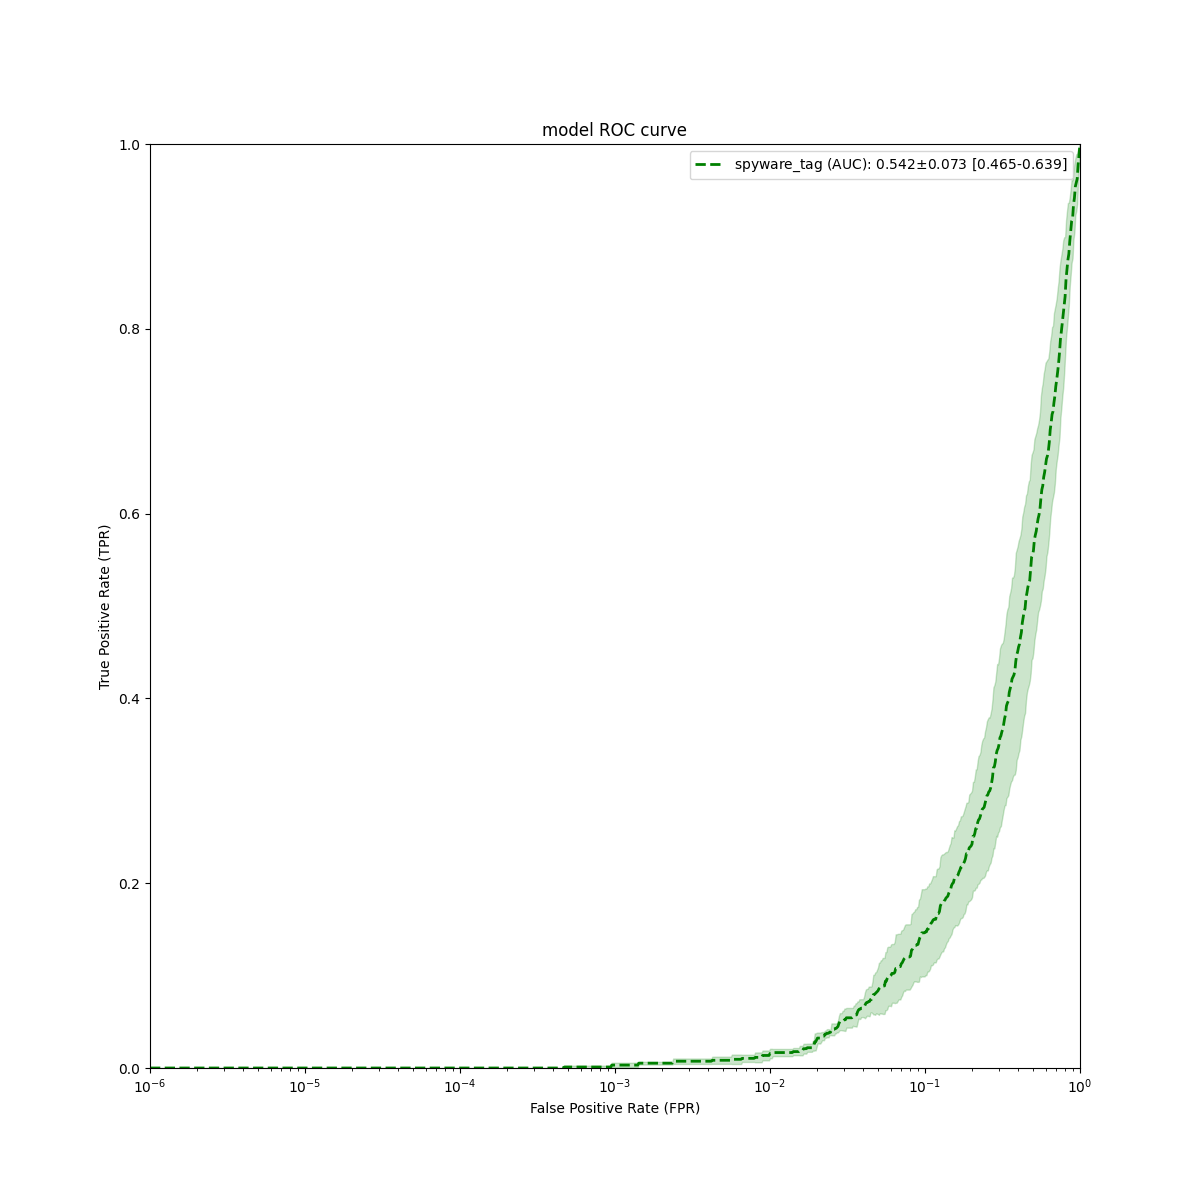
\includegraphics[width=0.6\textwidth]{./results/spyware_tag_roc_aloha.png}
        \vspace*{-0.2cm}
        \caption[Spyware Tag prediction task ALOHA ROC curve]{ROC curve and AUC statistics of \textBF{ALOHA} model for the \textbf{Spyware Tag}. The line represents the \textit{mean} TPR at a given FPR, while the shaded region represents the \textit{standard deviation}. Statistics were computed over \textBF{3} training runs, each with random parameter initialization.}
        \label{fig:spywareTagRocAloha}
    \end{figure}
}

\newcommand{\spywareTagRocJointEmbedding}{
    \begin{figure}[h!]
        \vspace*{-0.5cm}
        \centering
        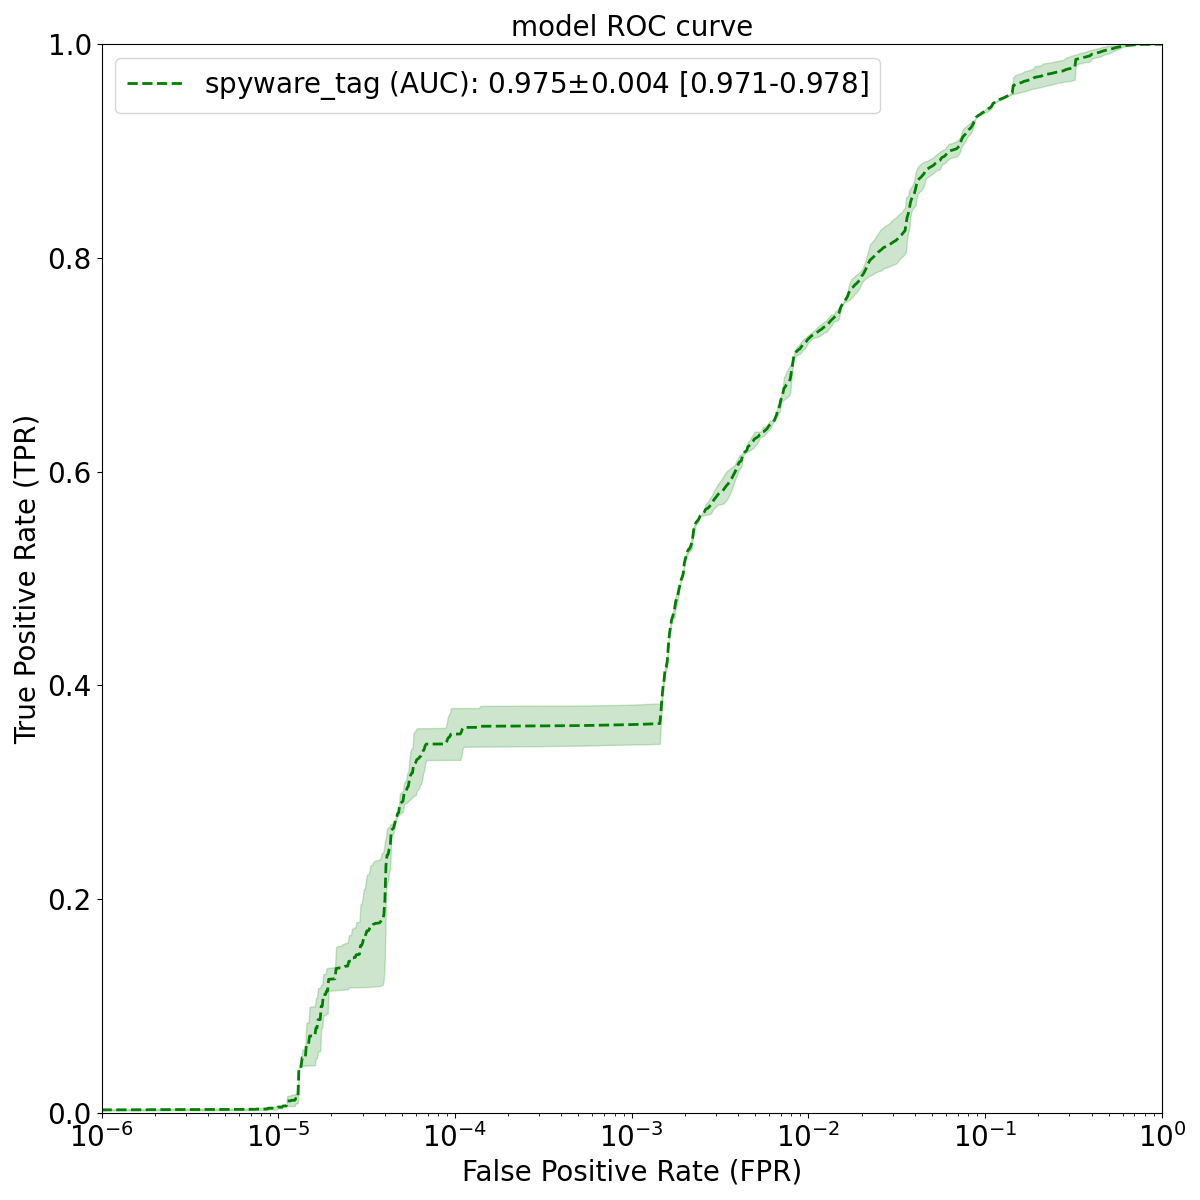
\includegraphics[width=0.6\textwidth]{./results/spyware_tag_roc_jointEmbedding.png}
        \vspace*{-0.2cm}
        \caption[Spyware Tag prediction task Joint Embedding ROC curve]{ROC curve and AUC statistics of \textBF{Joint Embedding} model for the \textbf{Spyware Tag}. The line represents the \textit{mean} TPR at a given FPR, while the shaded region represents the \textit{standard deviation}. Statistics were computed over \textBF{3} training runs, each with random parameter initialization.}
        \label{fig:spywareTagRocJointEmbedding}
    \end{figure}
}

\newcommand{\spywareTagRocProposedMethod}{
    \begin{figure}[h!]
        \vspace*{-0.5cm}
        \centering
        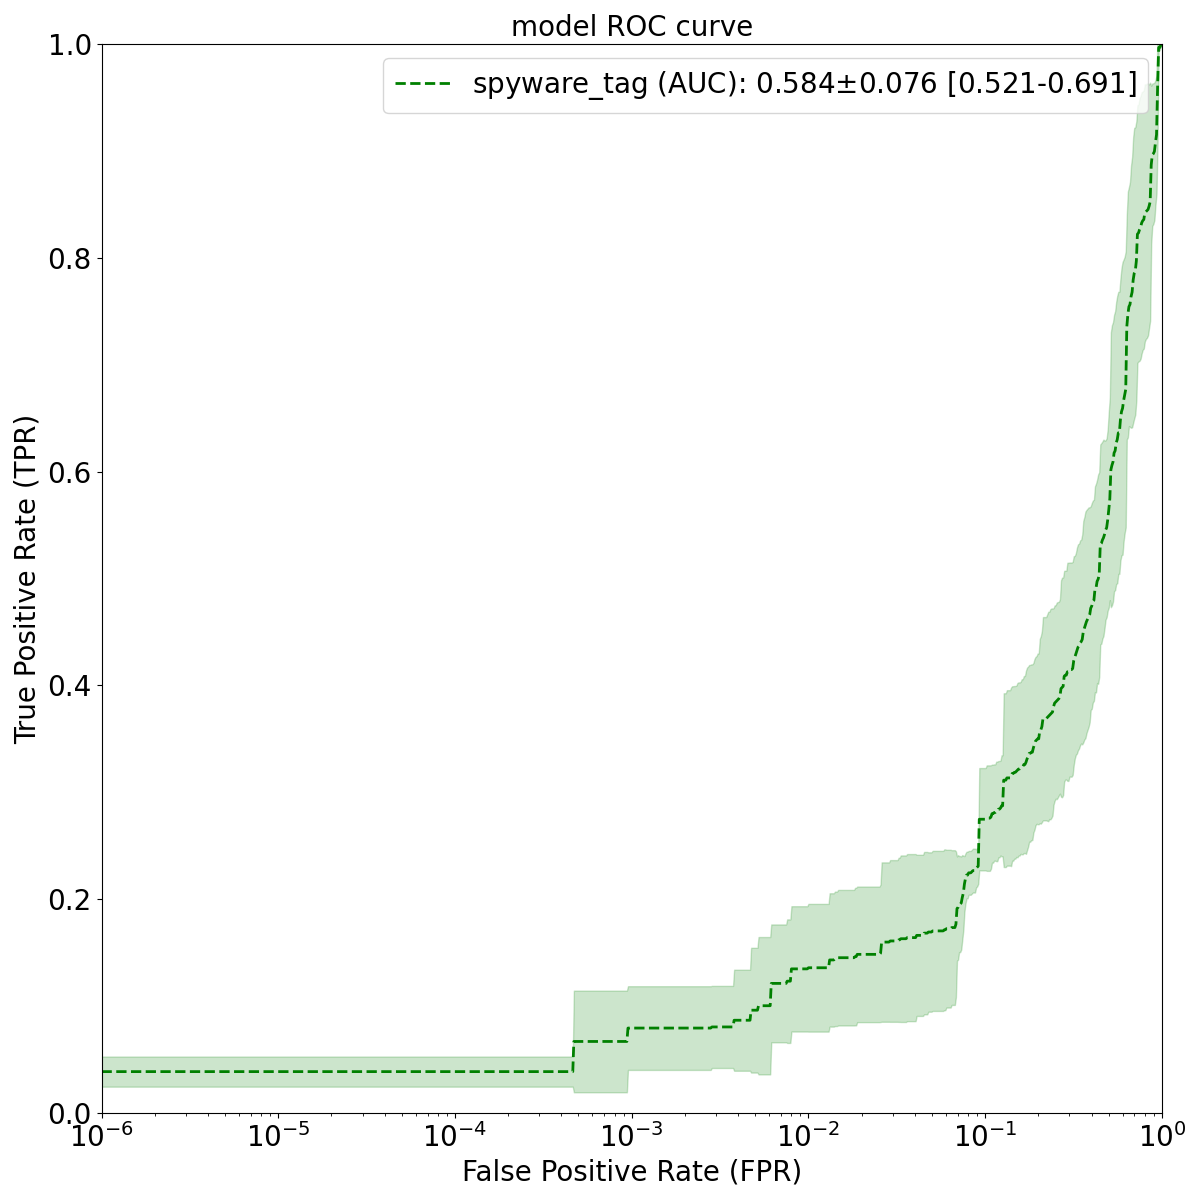
\includegraphics[width=0.6\textwidth]{./results/spyware_tag_roc_proposedModel.png}
        \vspace*{-0.2cm}
        \caption[Spyware Tag prediction task Proposed Model ROC curve]{ROC curve and AUC statistics of \textBF{Proposed Model} for the \textbf{Spyware Tag}. The line represents the \textit{mean} TPR at a given FPR, while the shaded region represents the \textit{standard deviation}. Statistics were computed over \textBF{3} training runs, each with random parameter initialization.}
        \label{fig:spywareTagRocProposedModel}
    \end{figure}
}
